\paragraph\
    There are many NetFlow collectors available as commercial products and open source products as well. We have used \emph{ntop}
    as our NetFlow collector for this project as it is an open source project and has the performance to handle traffic at 1Gbps rate with the \emph{libcap} library \cite{}.  %AP: cite here Luca Deri's doc/paper.
    \emph{ntop} uses a persistent database, RRDTool, which stores time series data. \emph{ntop}
    also stores NetFlow records into an in-memory data structure which is not a persistent data storage.  However, RRD has the drawback that it has a limited file size and treats it as a circular queue. This overwrites the data due to which historical information needed for data anlaytics is lost.
    
    \paragraph\
    We have extended \emph{ntop}
    with Cassandra, a NoSQL database which scales well as compared to other databases such as Redis \cite{} and HBase \cite{ha}  (see Fig. \ref{cassandrathpt}). \emph{ntop} extended to store data in Cassandra database provides the persistent storage required by our scalable flow monitoring
    solution. \emph{ntop} supports only C for writing a plugin. %AP: I am not sure this expression is correct.(Done)
    and there are no Cassandra clients written in C. Therefore we have developed a Cassandra  client in C
   which is explained in Section \ref{c_client}. We used this to develop the Cassandra plugin for $ntop$.
   
    \paragraph\
    This chapter is organized as follows: In Section \ref{ntop_section}, we present an overview of \emph{ntop} and its architecture.
    In Section \ref{why_section}, we present, in detail, the justification for choosing Cassandra as the persistent data storage for $ntop$. The Cassandra C client is explained in 
    section \ref{c_client}. Section \ref{cass-plugin} describes the implementation of Cassandra plugin for \emph{ntop}. Finally we conclude with Section \ref{chapter3_summary}.

\section{\emph{ntop}}\label{ntop_section}
  \emph{ntop} is an open source traffic measurement application written in C. \emph{ntop} design follows the UNIX Philosophy: applications can be divided into small independent pieces that co-operate to achieve a common goal. \emph{ntop} captures packets from the network with \emph{libcap} library and analyzes
  packets received from \emph{libcap}. \emph{ntop} architecture is shown in Fig.  \ref{ntop_architecture}. 
  
It consists of the following components:
    \begin{enumerate}
     \item Packet Sniffer - Captures packets using \emph{libpcap} library and also from UNIX sockets.
     \item Packet Analyzer - Analyzes packets captured by Packet Sniffer.
     \item Traffic Rules - \emph{ntop} allows traffic rules for capturing packets to filter out unnecessary packets.
     \item Report Engine - Report Engine displays analyzed output in an interactive web-based user interface. 
     \item Plugins - Using plugins anyone can extend \emph{ntop} to support extra features.
    \end{enumerate}

    Each of these components is implemented asynchronously by means of a thread.  We describe the function of each of these components in the rest of this section.

  \paragraph{Packet Sniffer}

	Packet Sniffer captures packets using \emph{libpcap} library and stores them into internal buffers. This helps to reduce packet drops in a bursty traffic environment. \emph{libpcap} is supported by all major operating systems. This allows \emph{ntop} to be portable to Windows and UNIX variants.

        \begin{figure}[htb]
          \centering
          \includegraphics[scale=.5]{ntoparc.jpg}
          \caption{Architecture of \emph{ntop}.} 
          \label{ntop_architecture}
        \end{figure}

	 \paragraph{Packet Analyzer}
	 Packet Analyzer gets packets from Packet Sniffer and processes those packets. Sniffed packets contain information about status of the network and that information is calculated by Packet Analyzer and then stored in RRD for future references.

	\paragraph{Traffic Rules}

	  \emph{ntop} allows the user to specify what kind of traffic a user is interested in. Using \emph{libpcap} filter expression 
	  \emph{ntop} achieves this goal. Traffic Rules help \emph{ntop} to reduce some burden on memory as well as the CPU and make \emph{ntop} faster as it processes less number of packets.

	\paragraph{Report Engine}

	  \emph{ntop} contains a web server by which users from any geographical location can configure and monitor their network.
	  Report Engine provides an interactive user interface with time series graph drawn using RRDTool. Using the Report Engine a user can change the behavior of \emph{ntop} by changing its configuration parameters.

	\paragraph{Plugins}
	 \emph{ntop} has a flexible design that allows users to add their own plugins. At startup \emph{ntop}
	 searches shared libraries (like .so, .dll files) to load  plugins. A plugin can access \emph{ntop}'s global 
	 data structures and can use API exported by \emph{ntop}.
	 
  \subsection{Issues with \emph{ntop}}
  \paragraph\
    \emph{ntop} uses round robin database called RRDTool for storing statistics. RRDTool stores time series data into flat files. We have to predefine the number of data points for our time series data during the creation of the RRDTool file. 
    
     Limitations of RRDTool are:
    \begin{enumerate}
       \item Data files generated by RRDTool are not machine independent.
       \item Time series data cannot be distributed over multiple files.
       \item Data file size is fixed at the time of creation.
      \end{enumerate}

    On the other hand \emph{ntop} uses in-memory data structure to store flow records reported by NetFlow packets which are deleted after a timeout. \emph{ntop} also deletes flow records
    if in-memory data structure crosses threshold size.

    \paragraph\ Because of these limitations we have added Cassandra support to \emph{ntop} to overcome current issues. In the next
    section we explain about reasons for choosing Cassandra as a persistent database.
    
    
 \section{Why Cassandra} \label{why_section}
      \paragraph\
	  In one of our testbeds we are able to generate approximately 1000 NetFlow packets per second with only two nodes
	  having 1 Gbps NIC card. Table \ref{datagenerated} provides the amount of data generated by our testbed.
	  
	  \begin{table}[ht]
	  \centering
	  \label{datagenerated}
	    \begin{tabular}{ccc}
	      \\
	      \hline
	      Packets generated& Time & Size of generated data \\
	      \hline
	      1000   & 1 second & 1.4MB\\
	      60 k   & 1 minute & 85 MB\\
	      3.6 m  & 1 hour    &  5 GB\\
	    \end{tabular}
	    \caption{Data generated by two node testbed.}
	    \label{datagenerated}
	   \end{table}
	  
	It is clear that we cannot use RDBMS based databases for storing flows in data center networks as they create huge amount of data in a short time. 

	The features required by a database for flow monitoring are:
	\begin{enumerate}
	  \item Scalability : So that huge amount of data can be stored according to the demand.
	  \item High write throughput : As flow records are generated at a rapid speed in data center networks, a flow monitoring system needs to write them fast.
	  \item Reasonable read performance : For real-time flow processing.
	  \item MapReduce support: For offline flow processing it needs to support MapReduce to enable massive data crunching operation.
	\end{enumerate}

	\paragraph{Redis:} Redis is written in C. It has fast read/write performance but is not scalable. Redis cluster, which is expected to support scalability, is going to be launched by the end of 2013 \cite{rrdcluster}. 
	\paragraph{HBase:} HBase is written in Java. It is scalable, has good read/write performance but is suitable only for batch processing. It has a single point of failure with Hadoop NameNode due to which HBase may lose data.

       \paragraph{Cassandra:} A performance test done by DataStax \cite{} shows that Cassandra performs more operations than Redis and Hbase. Figure \ref{cassandrathpt} from their report \cite{} illustrates claims of their test. Figure \ref{cassandrathpt} also shows scalability of Cassandra as 
	throughput increases with more number of Cassandra nodes. In the next section, we give a brief introduction to the architecture of Cassandra and its data model.

	\begin{figure}[htb]
	    \centering
	    \includegraphics[scale=.5]{cassathpt.png}
	    \caption{Cassandra Performance \cite{cassathpt}.} 
	    \label{cassandrathpt}
	  \end{figure}

      
\section{Cassandra Database}\label{cas}
\paragraph\
      Cassandra is a highly scalable and highly available database initially developed by Facebook using two famous approaches: Big Table \cite{bigtable} from Google and Dynamo \cite{dynamo} from Amazon. Cassandra is extensively used in ebay and Netflix. 

      Cassandra's Big Data features \cite{cassafeatures} are: 
      \begin{enumerate}
       \item Elastic scalability.
       \item High availability.
       \item Distributed database design with no single point of failure.
       \item Good linear performance.
       \item Multiple data center based data distribution.
      \end{enumerate}
      
      \subsection{Cassandra Architecture:}
      \paragraph\
      Cassandra runs on a cluster of commodity hardware. Cassandra cluster nodes form a ring topology to partition
      the data into multiple nodes. A Cassandra ring topology is illustrated in Figure \ref{cassandra_ring}. Each node in a Cassandra 
      ring acts as a peer node to implement peer-to-peer distribution model. Cassandra ring uses Gossip \cite{gossip} protocol for intra-ring
      communication. Gossip protocol helps to detect failure nodes in the Cassandra ring. Nodes can enter and exit the ring at various times without affecting the operation of Cassandra.
      
      \paragraph\ Any node in a Cassandra ring can process read/write requests. As independent Cassandra nodes can perform read/write operations,
      Cassandra improves its performance with addition of nodes into Cassandra ring. Read/write operations are done on dynamic schema 
      distributed in multiple Cassandra nodes.
      
%	  Cassandra has a peer-to-peer distribution model. Therefore all nodes in a Cassandra cluster are symmetric.
%	  Any node can take read/write requests from clients and forward them to the correct node in the cluster. This design makes 
%	  Cassandra scalable. Cassandra uses Gossip \cite{gossip} protocol for intra-ring communication to support decentralization and partition  tolerance.  % AP: What do you mean partition tolerance? Does not make sense to me. Likely it is partition fault tolerance? Check it out.
%	  Gossip protocol helps to detect failures and recovery of a Cassandra node as well. Cassandra which is also known as Cassandra ring
%	  illustrate in the figure \ref{cassandra_ring}. Cassandra cluster logically forms ring topology. Cassandra uses this ring topology to 
%	  shard the token range. This topology also used while replication, as all the replicated data from a node goes to next clockwise node.

	  \begin{figure}[htb]
		\centering
		\includegraphics[scale=.5]{cassandra_ring.png}
		\caption{Cassandra Ring \cite{cassandra_ring}} 
		\label{cassandra_ring}
	      \end{figure}
	 
	 %Figure \ref{Cassandra_ring} describe about a Cassandra ring.
	 %AP: Figures dont describe. they illustrate. Anyway, there is a real problem here in terms of the way you are writing about cassandra. If you read your doc., you will see that you have not mentioned anything about a ring in the architecture above. You suddenly use intra-ring which will make no sense to your reader who is not familiar with cassandra ring. So, the way to do it is to describe more about cassandra in terms of a ring and how it uses the ring and use the figure to illustrate this description. Hence, you need to re-write the whole cassandra arch. properly.
	 
	 \paragraph{Cassandra Data Model:}
	  Cassandra uses dynamic schema based column oriented data model. 
	  In a Dynamic schema we do not need to model all of the columns required by an application up front, as each row is not required to have the same set of columns.
	  A database in a Cassandra, called  a $keyspace$, consists of $column families$.
	  A $column family$ is a group of key-value pairs sorted by column name. A node in a Cassandra ring gets a token range at startup and gets 
	  ownership of all keys that fall into that token range. Keys in a column family are sorted according to the partition
	  of the Cassandra ring. There are two partitioning  schemes for a Cassandra ring:
	  \begin{enumerate}
	   \item  Random Partitioner: It uses a 128-bit MD5 hash value as a token. It is the default partitioning strategy that helps automatic load balancing as MD5 hash value ensures even key distribution.
	   \item Ordered Partitioner: It uses byte order of key as token. It allows range scan over rows. %AP: explain range scan.
	  \end{enumerate}

	  A Cassandra ring contains multiple $keyspaces$. Each $keyspace$ contains many column families distributed across the Cassandra ring.
	  Figure \ref{cassandra_data_model} illustrates a Cassandra data model consisting of a $keyspace$ containing two column families.
	  As Cassandra uses dynamic schema, number of columns in a row can be different from other rows. This is seen in the data model of Fig. \ref{cassandra_data_model}.
	  %illustrates dynamic schema of a Cassandra as well.\\

	  \begin{figure}[htb]
		\centering
		\includegraphics[scale=.5]{cassandra_data_model.png}
		\caption{Cassandra Data Model} 
		\label{cassandra_data_model}
	      \end{figure}

The table below compares RDBMS schema with Cassandra data model.\\
	  \begin{table}[ht]
	  \centering
	   \begin{tabular}{|l|l|}
	   \hline
	   {\bf RDMS}     & {\bf Cassandra}      \\ \hline 
	   Database & Keyspace       \\
	   Table    & Column Falily  \\
	   Entity   & Column Name    \\
	   Value    & Column Value   \\ \hline
	  \end{tabular}
	  \caption{Comparison between RDMS schema with Cassandra Data Model}
	  \end{table}

	  \paragraph{Memtables, SSTables and commit log:}
	    Cassandra uses in-memory data structures called memtables for caching recent writes to a Cassandra node.
	    Memtables are later stored into disk as SSTables depending on timeout or  memtable threshold size.
	    On crash or on Cassandra node failure Commit log helps to recover data.	    

	    \paragraph{Read/Write Operation on Cassandra} Cassandra  uses the following steps for a write operation:
	    \begin{enumerate}
	     \item Write row values into commit log.
	     \item Write row values into memtable.
	     \item Persisit  memtables as SSTables on the disk.
	    \end{enumerate}
	    
	    While reading from Cassandra, a node first checks its memtable for the row. If the row is not found in the memtable, then all SSTables containing
	    the row have to be merged to get the whole row (as row value is distributed in multiple SSTables). Because of this merging operation Cassandra's read operations are slower than write operations. Cassandra maintains ``row cache'' and ``key cache'' to make read operations faster.
	    ``row cache'' and ``key cache'' are in-memory data structures to keep whole rows and location of the row keys respectively.

	    Figure \ref{cassandra_rw} illustrates read/write operations on a Cassandra node.
	      \begin{figure}[htb]
		\centering
		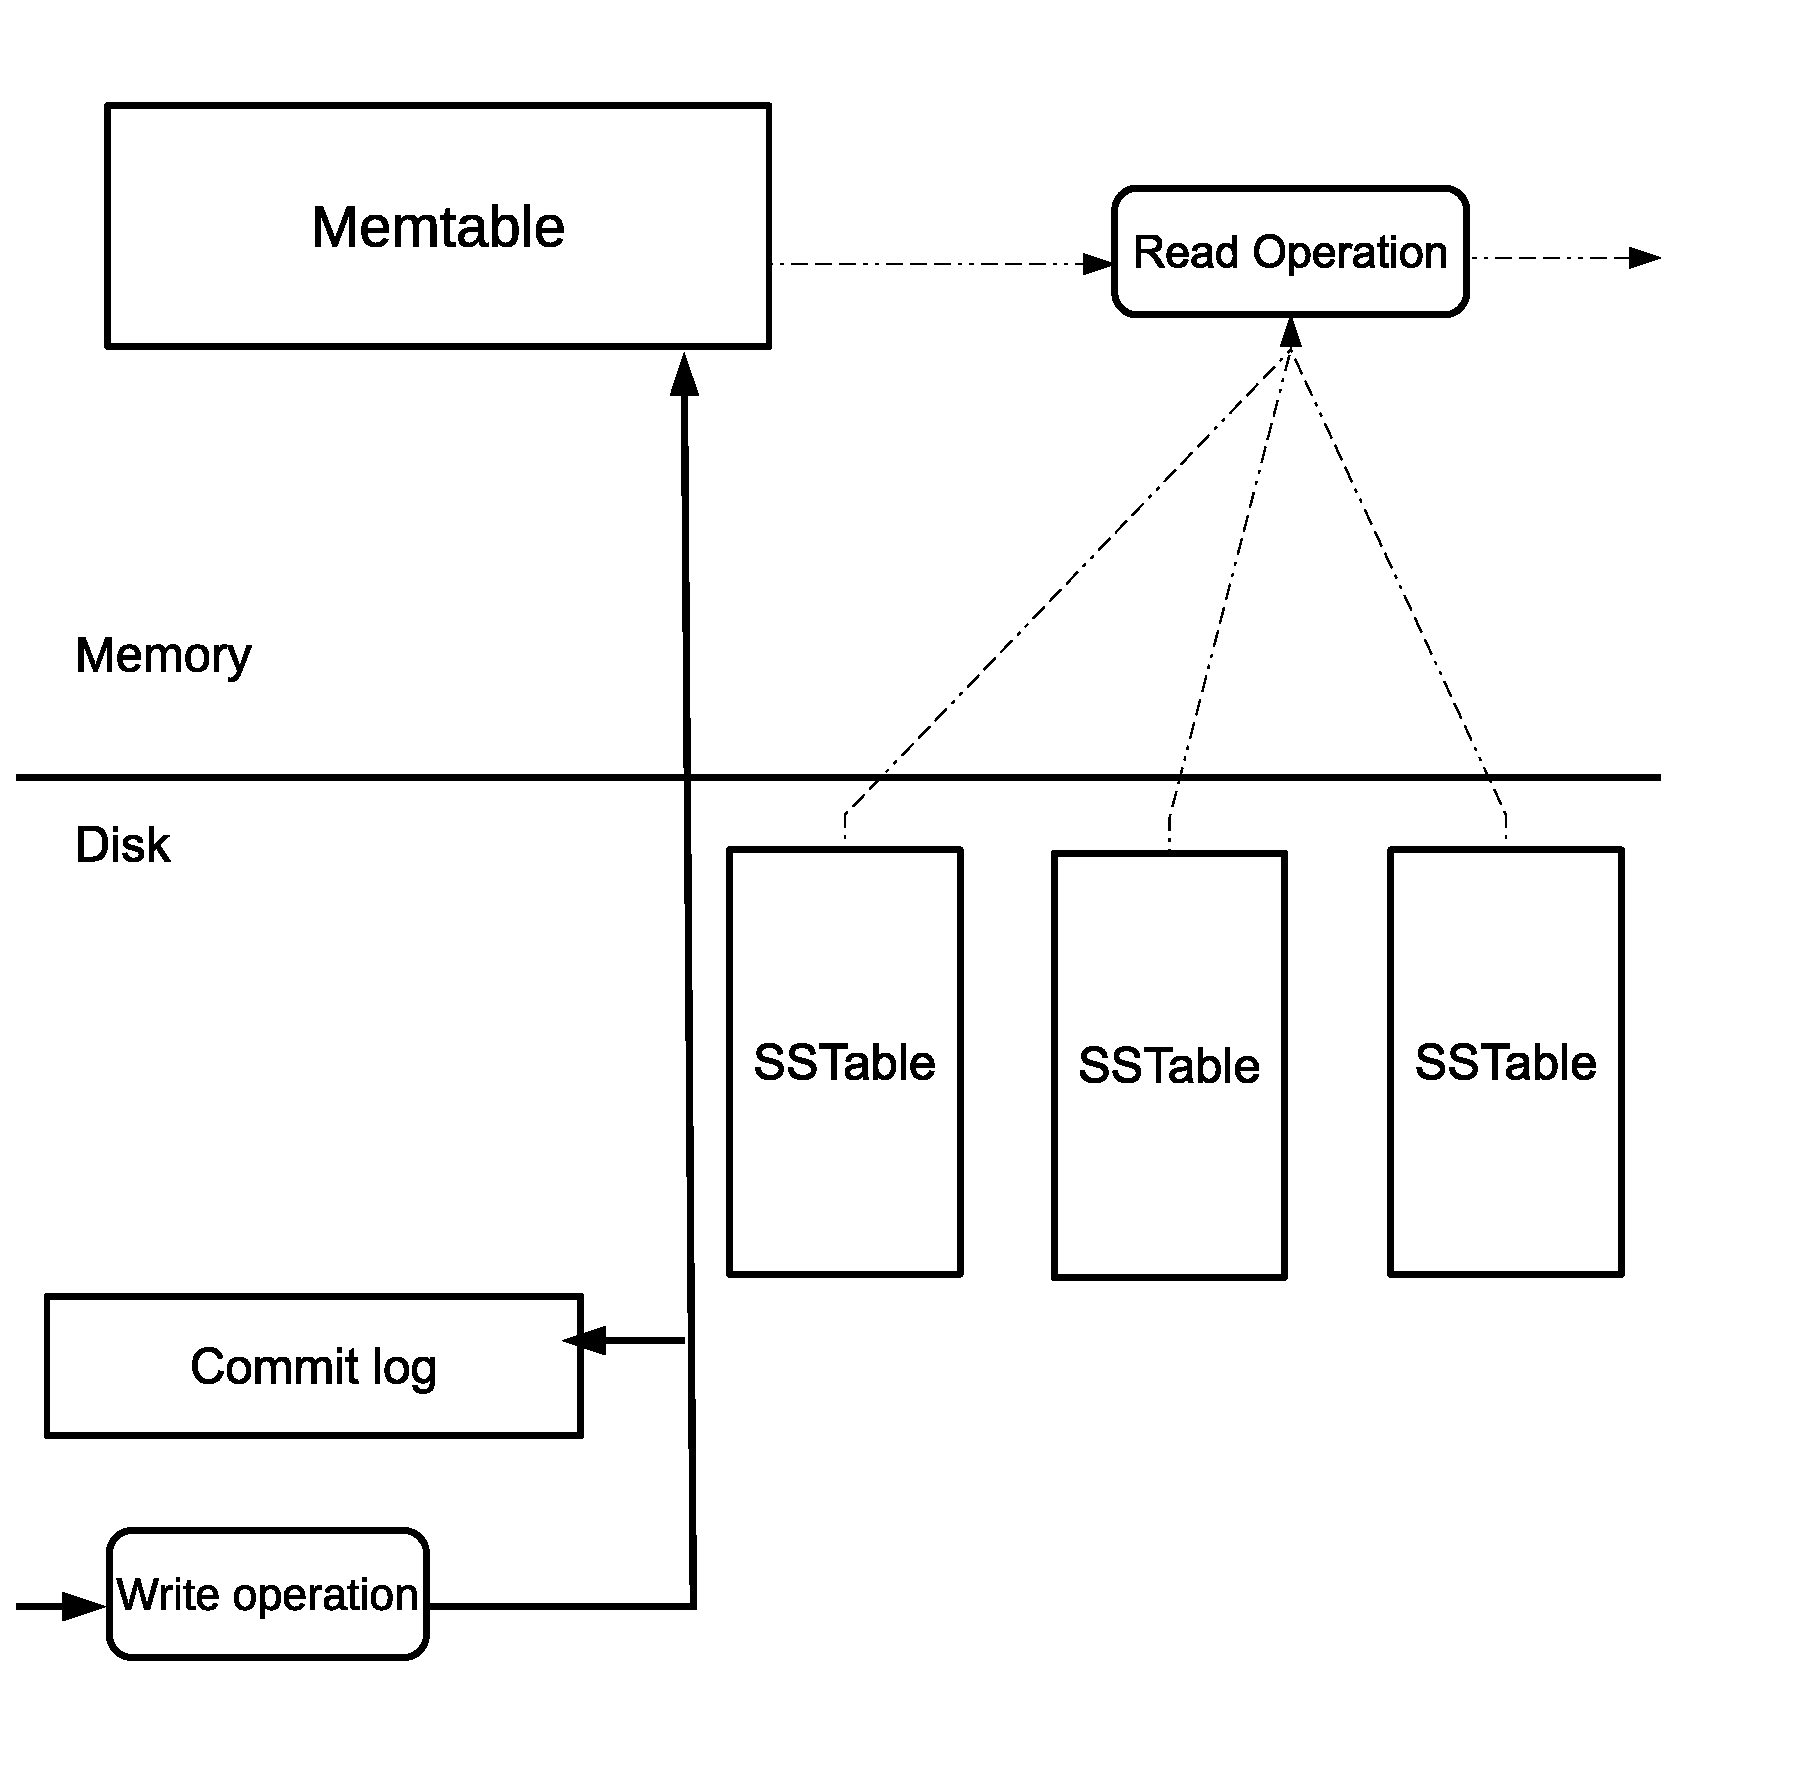
\includegraphics[scale=.35]{cassandra_rw}
		\caption{Cassandra Read/Write operation} 
		\label{cassandra_rw}
	      \end{figure}

    \paragraph\
    Cassandra has clients written in Java and Python but not C. \emph{ntop} uses only C for writing
    a plugin. Cassandra uses $thrift$ protocol for programming language independent interface. Developing a C client using thrift needs 
    plenty of time. So we decided to write a C wrapper API  for Cassandra on top of the Python client API, $Pycassa$.
    In the next section we describe our Cassandra C client.
    
\section{Cassandra C Client} \label{c_client}
\paragraph\
      Cassandra C client is a wrapper developed by me around Cassandra Python client, $Pycassa$. This allows any user to call Cassandra API from a C program.
Pycassa uses $thrift$ RPC call to communicate with Cassandra. Fig. \ref{cass-c-api} shows the architecture of the Cassandra C API.
      
Cassandra C client API has three major classes of APIs. These are :
      \begin{enumerate}
       \item Schema Manipulation API: Manages schema definitions of Cassandra.
       \item Data Manipulation API: Inserts or retrieves data from Cassandra. 
       \item Utility API:  API that do some common useful work. 
      \end{enumerate}

      \begin{figure}[htb]
	 \centering
         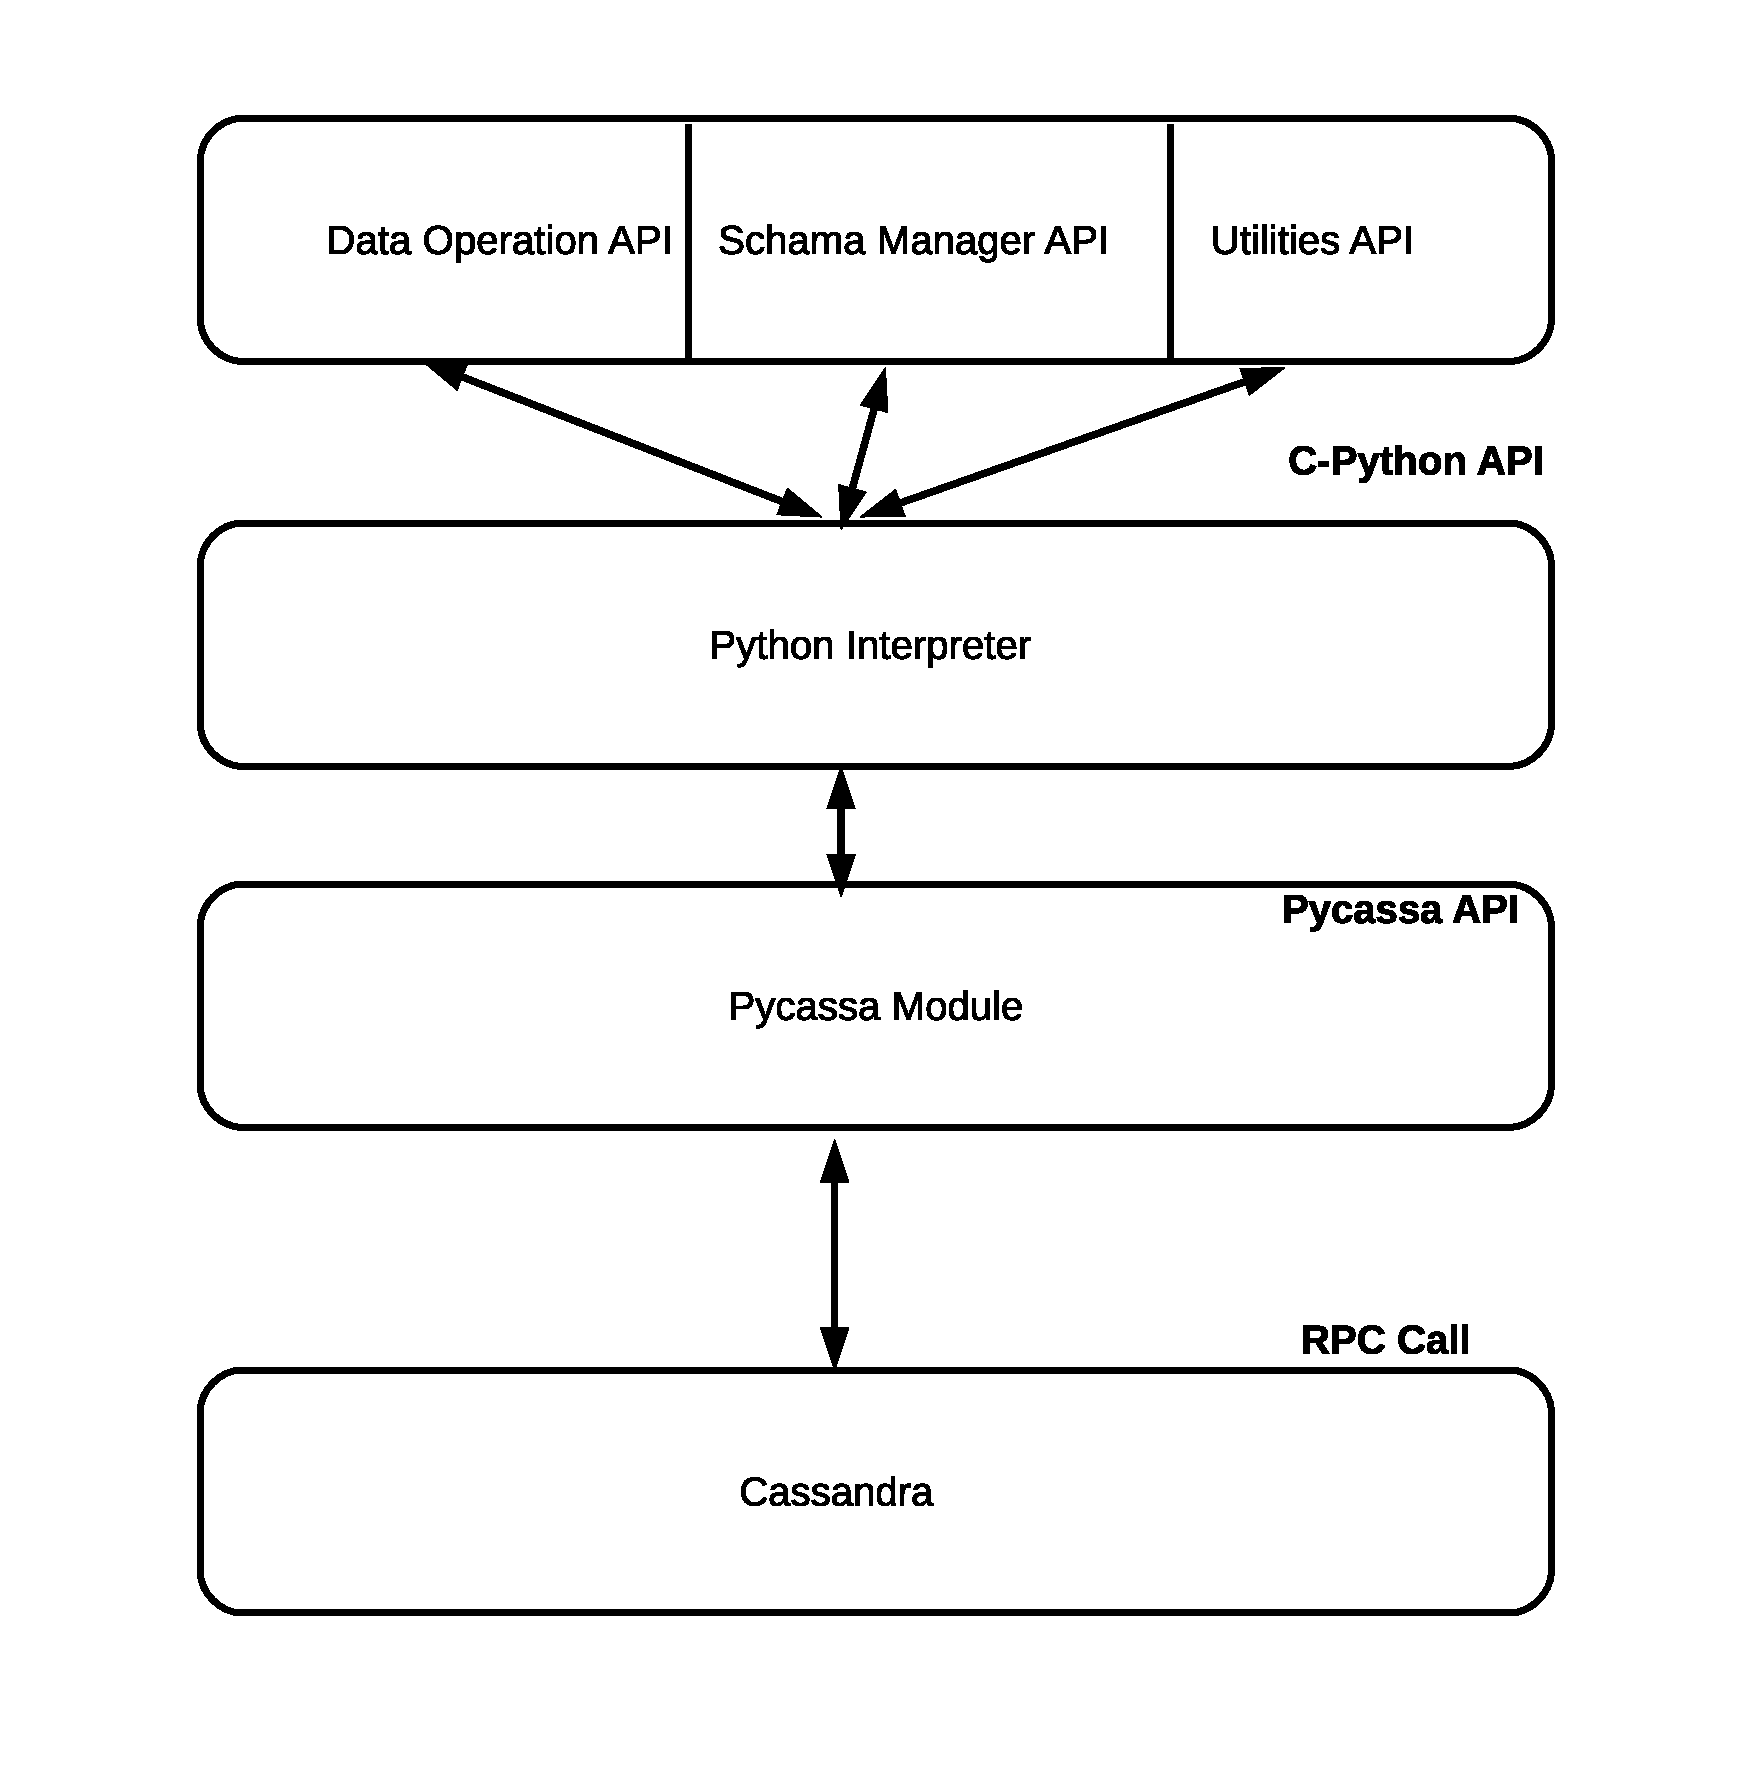
\includegraphics[scale=0.3]{C_client}
         \caption{API interaction with Cassandra }
	\label{cass-c-api}
      \end{figure}

\subsection{Schema Manipulation API}
      \paragraph\
      These APIs allow one to create or delete keyspace and column families. 

      \begin{enumerate}
       \item {\bf cassandraCreateKeyspace}(name, server, rf, strategy): Creates a keyspace on the server with the given replication factor(rf) and strategy.
	    Supported strategies are :
	     \begin{enumerate}
	      \item SimpleStrategy : Replication strategy that simply chooses consecutive nodes in the ring for replicas.
	      \item NetworkTopologyStrategy : Replication strategy that puts a number of replicas in each data center.
	      \item OldNetworkTopologyStrategy : OldNetworkTopologyStrategy is provided for backwards compatibility with old Cassandra installations.
	     \end{enumerate}

       \item {\bf cassandraCreateColumnFamily}(name, keyspace, comparator, server): Creates a column family, $name$, in the keyspace with the given comparator. 
	      Supported comparators are :
		    \begin{enumerate}
		     \item AsciiType
		     \item DoubleType
		     \item IntegerType
		     \item BytesType
		     \item LongType
		     \item FloatType
		     \item TimeUUIDType
		    \end{enumerate}

      \item {\bf cassandraDropColumnFamily}(name, keyspace, server): Deletes the given column family, $name$, from the keyspace.

      \item {\bf cassandraDropKeyspace}(name, server): Deletes keyspace, $name$, from the server.
      \end{enumerate}

    \subsection{Data Manipulation API}
    \paragraph\
    These APIs deal with insertion and retrieval of data from the Cassandra server.

      \begin{enumerate}
       \item {\bf cassandraConnect}(keyspace, columnfamily, server): Creates a connection and stores the connection object in the internal Python dictionary for later use. As connection creation takes time, connection objects are cached in the Python dictionary.

       \item {\bf cassandraInsert}(id, key, value, column name): Inserts a key-value pair in the column family referred by $id$.
       
       \item {\bf cassandraTimeSeriesInsert}(keyspace, cf, server, key, column\_name, value): Cassandra is heavily used as a
	      time series database because of its write performance. cassandraTimeSeriesInsert is a simplified way of inserting 
	      time series data into Cassandra. It stores $value$ into the column given by $column\_name$ in the column family, 
	      $cf$ as a time series data point.
	      This operation
	      uses an in-memory dictionary to cache recent connection objects to optimized write operation.

       \item {\bf cassandraGet}(id, key): Returns a dictionary of key-value pairs from  the column family referred by $id$.

       \item {\bf cassandraGetItem}(dictionary, position, name, value): Returns $name$/$value$ pair from given $position$ of the $dictionary$.  
      \end{enumerate}

    \subsection{Utility API}
    \paragraph\
    These APIs provide general functionality that we need.

      \begin{enumerate}
       \item {\bf isExistPycassa}(): It checks for the existence of $pycassa$ in the system.
       \item {\bf isExistKeyspace}(name, server): It checks for the existence of keyspace, $name$, on the server. 
       \item {\bf isExistColumnfamily}(name, keyspace, server): It checks for the existence of columnfamily, $name$, in the $keyspace$. 
      \end{enumerate}

      \paragraph\
      We have used our C client to store NetFlow records as well statistics calculated by \emph{ntop} into Cassandra. We describe the Cassandra plugin for \emph{ntop} in the next section.

      \section{Cassandra Plugin for \emph{ntop}}
      \label{cass-plugin}
      \paragraph\
      Cassandra Plugin is developed in C as a shared object. \emph{ntop} uses  the principle of shared objects to provide plugins, that allows dynamic linking of compiled shared objects  to \emph{ntop} to add extra features.

      \subsection{Architecture}
      Figure \ref{cassandraArch} illustrates our Cassandra Plugin architecture. Our Cassandra Plugin for \emph{ntop} stores all statistics in a Cassandra keyspace using cassandraTimeSeriesInsert() API. We have used cassandraTimeSeriesInsert() API for \emph{ntop}'s NetFlow module to store NetFlow records into Cassandra to get persistent storage.      
      Figure \ref{datamodel} shows the data model used by cassandraTimeSeriesInsert() API. TimeUUID is the data type for
      a key in the \emph{data} column family. Unix timestamp is not useful when time series data events occur at the same time. TimeUUID gives 
      a unique value even for the events that are generated at the same timestamp. Keyspace prefix provided in configuration file helps to resolve any collision. It is preferable to use UUID as a keyspace prefix. \emph{ntop} has multiple counters
      for every interface that it monitors. Counters are stored into their own column family created by \emph{ntop}.
      \begin{figure}[htb]
            \centering
            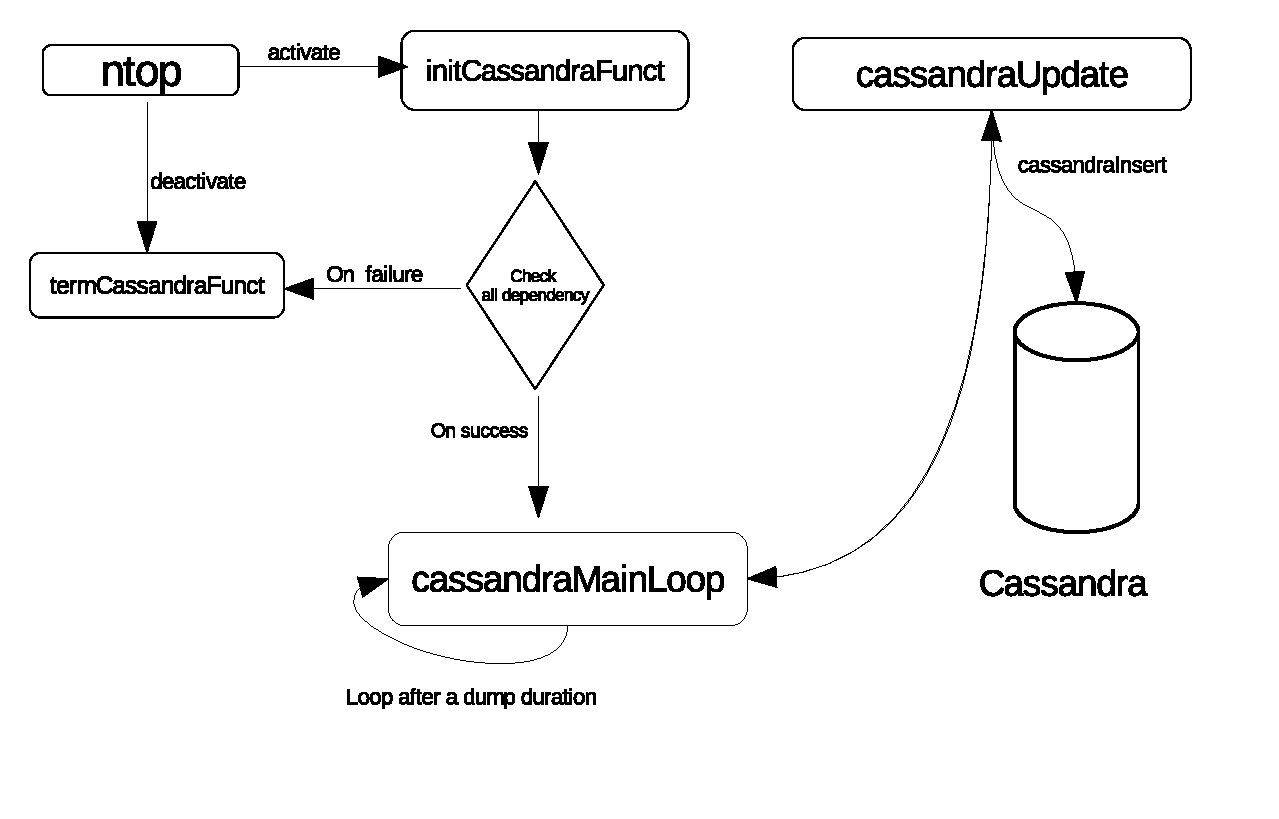
\includegraphics[scale = .7]{lfc}
            \caption{Architecture of Cassandra Plugin.} 
            \label{cassandraArch}
      \end{figure}
      \\
      \textbf{The APIs supported by \emph{ntop} for plugin support are given below:}\\
      \begin{table}[ht]
	\centering
	
	\label{ntopplugin}
	\begin{tabular}{|l|l|}
	    \hline
	    \textbf{API name} &  \textbf{Details}\\
	    \hline
	    int(*IntFunct)(void); & Called at initialization of the plugin.\\
	    \hline
	    void(*VoidFunct)(u\_char); & Called at termination of the plugin.\\
	    \hline
	    void(*PluginHTTPFunct)(char* url); & HTTP request handler function.\\
	    \hline
	  \end{tabular}
	  \caption{APIs for Plugin Support}
      \end{table}      

      \paragraph{API of Cassandra Plugin:} Given below are the APIs developed by me for a
      Cassandra Plugin for \emph{ntop}.\\
      
      \begin{enumerate}
       \item {\bf initCassandraFunct } (void): Initialize Cassandra Plugin. It checks for the $pycassa$ module, 
	      availability of the Cassandra server and then invokes cassandraMainLoop.
       \item {\bf termCassandraFunct} (u\_char termNtop): Terminates Cassandra Plugin.
       \item {\bf handlecassandraHTTPrequest} (char *\_url): It gets a web request from the web browser and serves them.\\
       \item {\bf cassandraMainLoop}(void) : This API does all the major work as described below:
	      \begin{enumerate}
	      \item Reads configuration files and initializes the data structure needed to store data.
	       \item Identifies sniffed interface, gets statistics from global variables and stores into Cassandra.
	       \item Identifies NetFlow socket, gets data from global variables and stores them to Cassandra. 
	      \end{enumerate}
      \end{enumerate}


      \begin{figure}[htb]
	    \centering
	    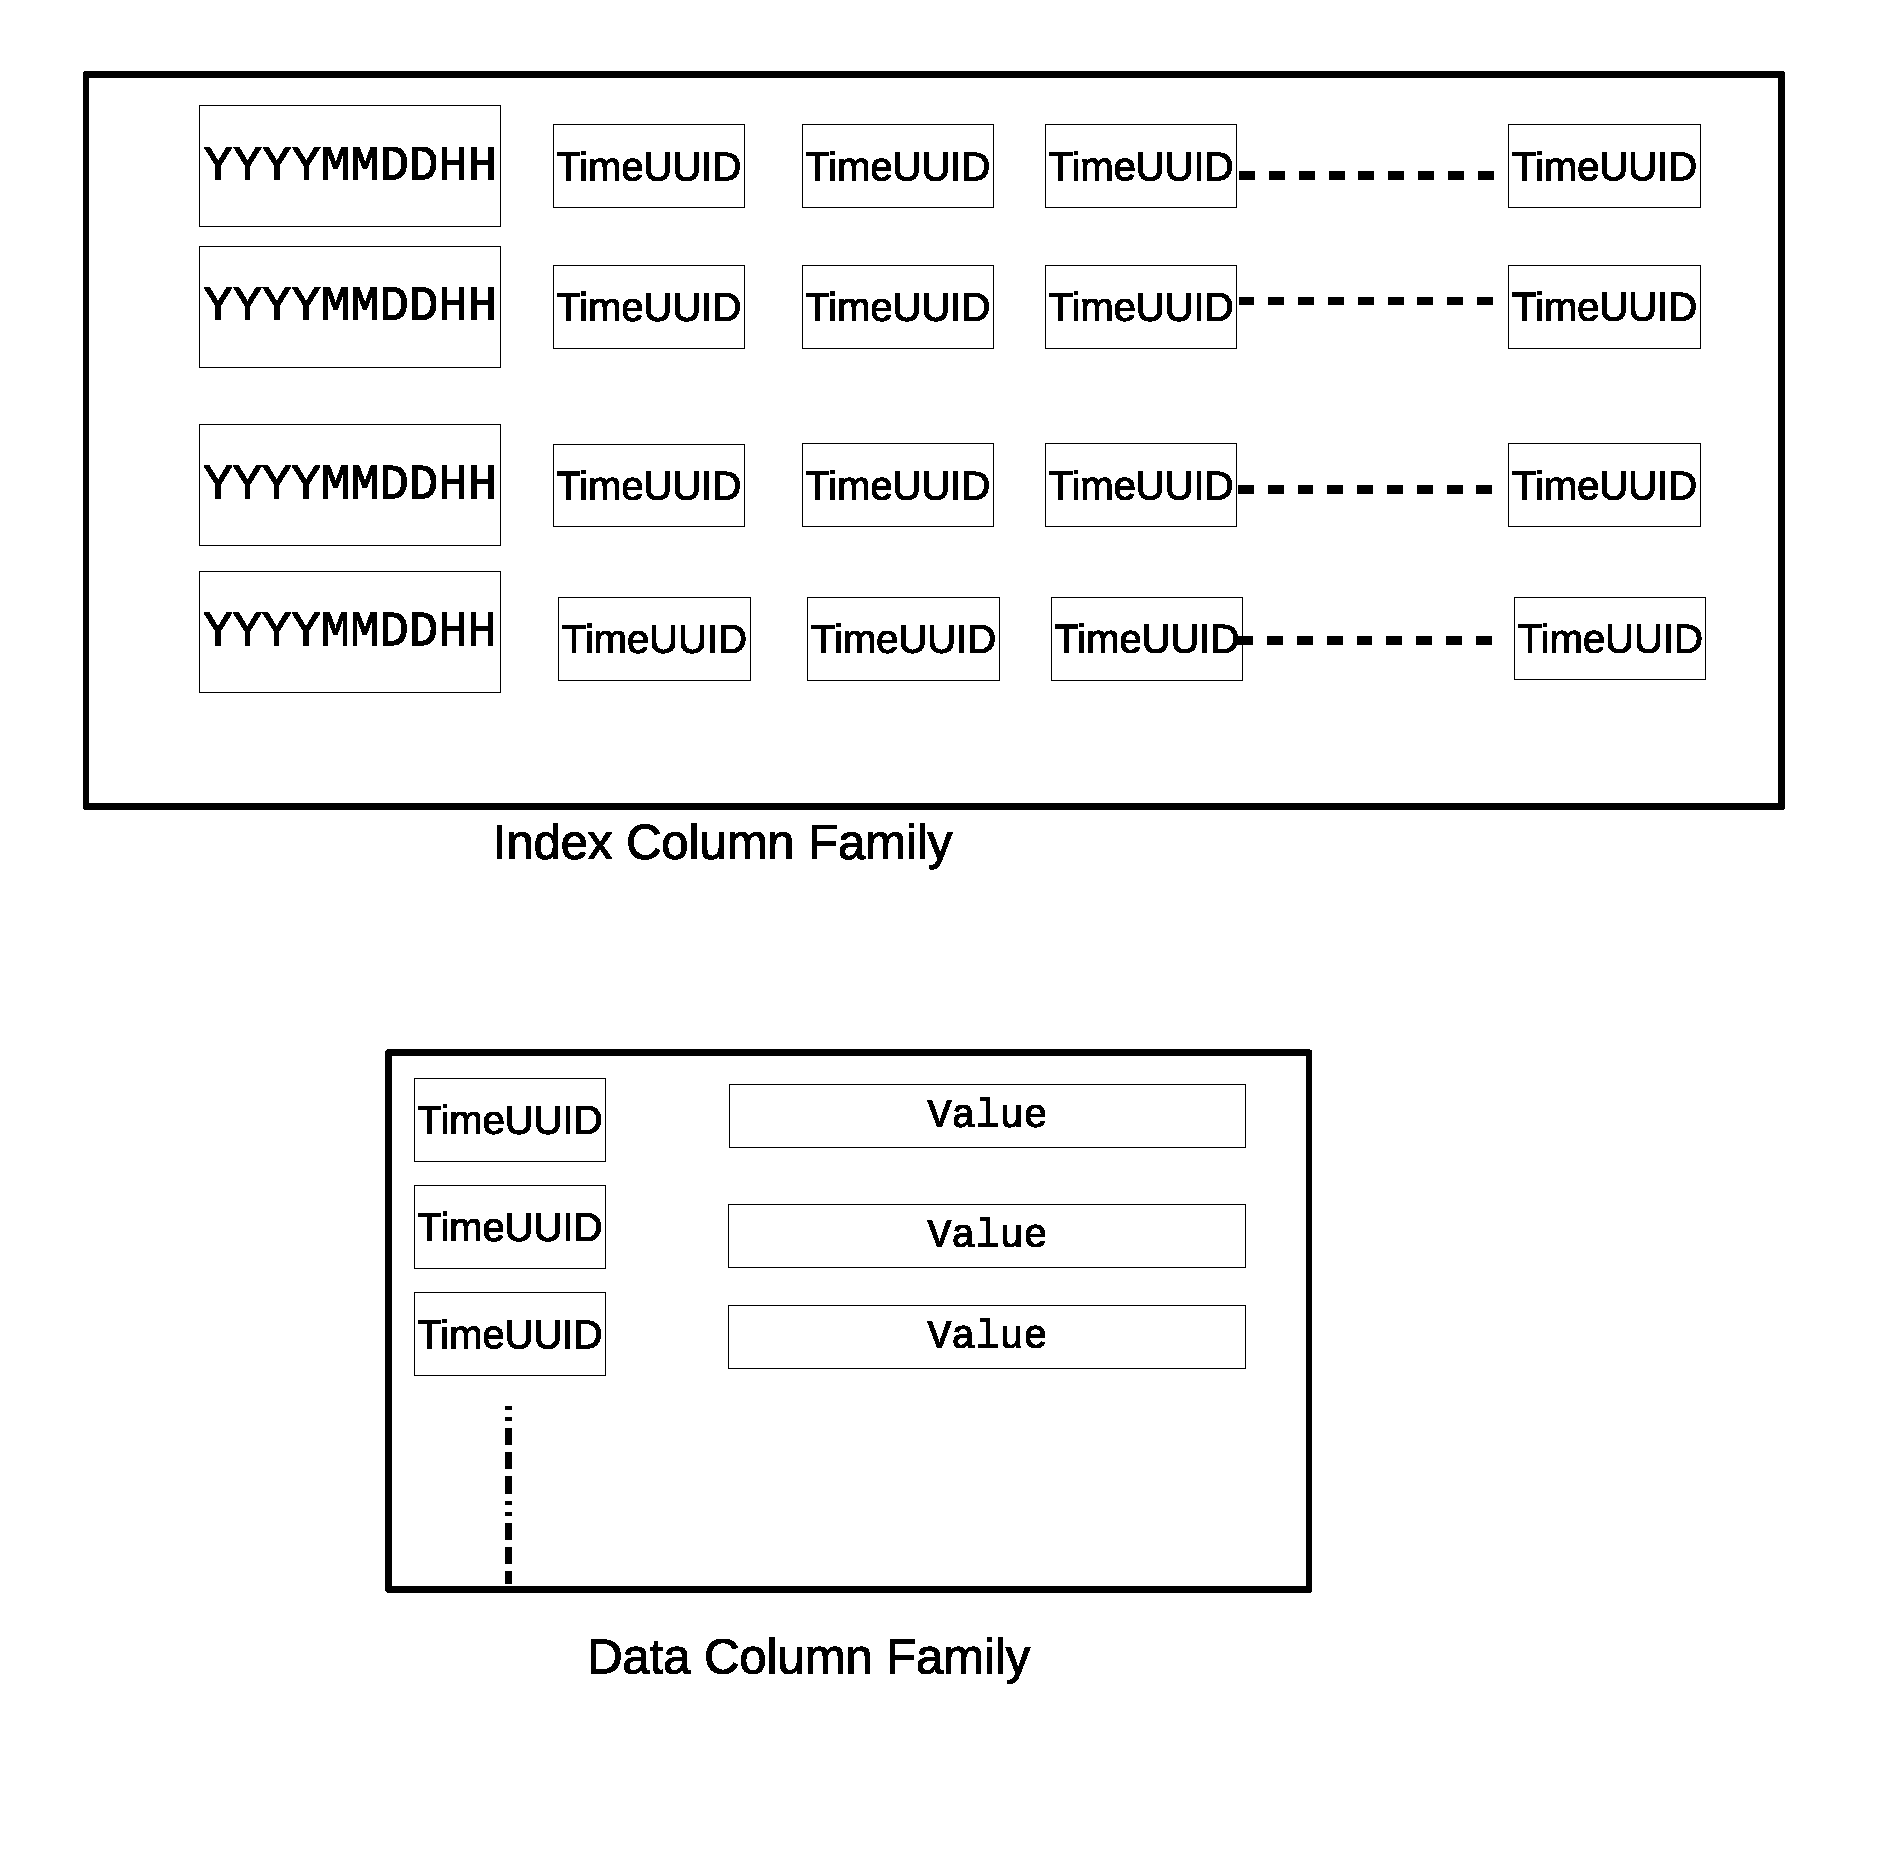
\includegraphics[scale = .4]{data_model}
	    \caption{Data Model for Cassandra \emph{ntop} Plugin.} 
	    \label{datamodel}
	  \end{figure}
	  
\section{Summary}\label{chapter3_summary}
\paragraph\
In this chapter, we have discussed the architecture and limitations of \emph{ntop} in terms of its capability to provide scalable and persistent storage for NetFlow records. We presented the features of Cassandra that make it an appropriate choice for scalable storage. Since Cassandra does not have a C client, we built a C wrapper API around its Python API, \emph{Pycassa}. We, then, extended \emph{ntop} to use Cassandra as the persistent storage by developing a plugin.

After testing the Cassandra plugin, we felt that NetFlow collectors such as \emph{ntop} cannot scale for the sort of traffic that may be observed in a data center. They represent single points of failure that violate the high availability requirement. Multiple NetFlow collector instances can be used to improve scalability as well as high availability. But, this leads to a replication of the features already built into Big Data databases such as Cassandra. One possible solution to this scalability issue is to let the NetFlow clients write directly to scalable databases. To test this hypothesis, we extended the NetFlow client of OpenVswitch to write directly to Cassandra instead of sending data to the NetFlow collector. This work is presented in the next chapter.